%  sample eprint article in LaTeX           --- M. Peskin, 9/7/00
%  modified for CTD2020, ctd2020-loc@iris-hep.org
%  This file is part of a tar file, which can be downloaded from the CTD2020 indico site. 
%  https://indico.cern.ch/event/742793/
%
\documentclass[10pt, paper=a4, UKenglish]{article}
\usepackage{graphicx}
\usepackage{textcomp}
\usepackage{array}
\usepackage{lineno}
\usepackage{url}
\def\UrlBreaks{\do\/\do-}

\linenumbers
%
%%%%%%%%%%%%%%%%%%%%%%%%%%%%%%%%%%%%%%%%%%%%%%%%%%%%%%%%%%%%%%%%%%%%%%%%%%%%
%   document style macros
%%%%%%%%%%%%%%%%%%%%%%%%%%%%%%%%%%%%%%%%%%%%%%%%%%%%%%%%%%%%%%%%%%%%%%%%%%%%
\def\Title#1{\begin{center} {\Large #1 } \end{center}}
\def\Author#1{\begin{center}{ \sc #1} \end{center}}
\def\Address#1{\begin{center}{ \it #1} \end{center}}
\def\andauth{\begin{center}{and} \end{center}}
\def\submit#1{\begin{center}Submitted to {\sl #1} \end{center}}
\newcommand\pubblock{\rightline{\begin{tabular}{l} Proceedings of CTD 2020\\ \pubnumber\\
         \pubdate  \end{tabular}}}

\newenvironment{Abstract}{\begin{quotation} \begin{center} 
             \large ABSTRACT \end{center}\bigskip 
      \begin{center}\begin{large}}{\end{large}\end{center} \end{quotation}}

\newenvironment{Presented}{\begin{quotation} \begin{center} 
             PRESENTED AT\end{center}\bigskip 
      \begin{center}\begin{large}}{\end{large}\end{center} \end{quotation}}

\def\Acknowledgements{\bigskip  \bigskip \begin{center} \begin{large}
      \bf ACKNOWLEDGEMENTS \end{large}\end{center}}

%%%%%%%%%%%%%%%%%%%%%%%%%%%%%%%%%%%%%%%%%%%%%%%%%%%%%%%%%%%%%%%%%%%%%%%%%%%% 
%  personal abbreviations and macros
%    the following package contains macros used in this document:
\input econfmacros.tex
%%%%%%%%%%%%%%%%%%%%%%%%%%%%%%%%%%%%%%%%%%%%%%%%%%%%%%%%%%%%%%%%%%%%%%%%%%%

\textwidth=6.5in
\textheight=8.75in
\hoffset=-0.85in
\voffset=-0.6in

%%  DO NOT CHANGE anything above.

% include packages you will need
\usepackage{color}
\usepackage{lineno}
\usepackage{subfig}
\usepackage{hyperref}

%%%%%%%%%%%%%%%%%%%%%%%%%%%%%%%%%%%%%%%%%%%%%%%%%%%%%%%%%%%%%%%%%%%%
% basic data for the eprint:
%%%%%%%%%%%%%%%%%%%%%%%%%%%%%%%%%%%%%%%%%%%%%%%%%%%%%%%%%%%%%%%%%%%%

%% preprint number data:
% Please replace XX by your contribution number in indico (a number between 01 to 62)
\newcommand\pubnumber{PROC-CTD2020-16}

%% date
\newcommand\pubdate{\today}

%%  Affiliation
\def\affiliation{
CERN, Geneva, Switzerland
}

%% Acknowledge the support
\def\support{\footnote{Work supported by Micron Technology, Inc.}}

%%%%%%%%%%%%%%%%%%%%%%%%%%%%%%%%%%%%%%%%%%%%%%%%%%%%%%%%%%%%%%%%%%%%%%%%%%%% 

\newcommand{\conference}{Connecting the Dots Workshop (CTD 2020)\\
April 20-30, 2020}

\usepackage{fancyhdr}
\pagestyle{fancy}
\definecolor{mygrey}{RGB}{105,105,105}
\fancyhf{} % sets both header and footer to nothing
\renewcommand{\headrulewidth}{0pt}
% \fancyhead[R]{\fontsize{8}{9} \color{mygrey} \selectfont  CTD 2020 \\}
\fancyhead[C]{\fontsize{7}{8} \color{mygrey} \selectfont Connecting
  the Dots. April 20-30, 2020\\}
\fancyfoot[C]{\thepage}

%%%%%%%%%%%%%%%%%%%%%%%%%%%%%%%%%%%%%%%%%%%%%%%%%%%%%%%%%%%%%%%%%%%%

\begin{document}

% uncomment the following line for adding line numbers
% \linenumbers

% large size for the first page
\large
\begin{titlepage}
\pubblock

%% Change the title, name, abstract
%% Title 
\vfill
\Title{40 MHz Scouting with Deep Learning in CMS}
\vfill

%  if you need to add the support use this, fill the \support definition above. 
%  \Author{FIRSTNAME LASTNAME \support}
%Hannes, Dinyar, Petr (FNAL), Konstantinos, Manos
\Author{Dejan Golubovic\footnote[1]{Corresponding author}, Thomas Owen James, Emilio Meschi, Ema Puljak, on belhalf of the CMS Colaboration}
\Address{\affiliation}
\vfill

\begin{Abstract}
A 40 MHz scouting system at CMS would provide fast and virtually unlimited statistics for detector diagnostics, alternative luminosity  measurements and, in some cases, calibrations, and it has the potential to enable the study of otherwise inaccessible signatures, either too common to fit in the L1 accept budget, or with requirements which are orthogonal to `mainstream' physics, such as long-lived particles.
Deep learning is a class of machine learning algorithms that uses multiple layers to progressively extract higher-level features from the raw inputs. A series of studies on different aspects of LHC data processing have demonstrated the potential of deep learning for CERN applications. The usage of deep learning aims at improving physics performance and reducing execution time.
This talk will present a deep learning approach to muon scouting in the Level-1 Trigger of the CMS detector. The idea is to utilize multilayered perceptrons to `re-fit' the Level-1 muon tracks, using fully reconstructed offline tracking parameters as the ground truth for neural network training. The network produces corrected helix parameters (transverse momentum, $\eta$ and $\phi$), with a precision that is greatly improved over the standard Level 1 reconstruction. The network is executed on an FPGA-based PCIe board produced by Micron Technology, the SB-852. It is implemented using the Micron Deep Learning Accelerator inference engine. The methodology for developing deep learning models will be presented, alongside the process of compiling the models for fast inference hardware. The metrics for evaluating performance and the achieved results will be discussed.
\end{Abstract}

\vfill

% DO NOT CHANGE!!!
\begin{Presented}
\conference
\end{Presented}
\vfill
\end{titlepage}
\def\thefootnote{\fnsymbol{footnote}}
\setcounter{footnote}{0}
%

% normal size for the rest
\normalsize 

%% Your paper should be entered below. 

\section{Introduction to 40 MHz Scouting}
\label{Introduction}
%comments from TJ - need reference for original CMS e.g original CMS document. Need reference for lumi statements

Collisions in the Large Hadron Collider (LHC), which occur at a bunch crossing (BX) rate of 40 MHz, generate huge amounts of data in the detectors. The Compact Muon Solenoid (CMS)~\cite{tdr} detector contains $\sim$10\textsuperscript{8} electronic channels, making reading out and analysing every channel at the full BX rate unfeasible. This promotes the need for a triggering system to select the events to be read out for analysis. A two-tiered trigger system is used. The first stage is the Level-1 (L1) trigger~\cite{trigger}, implemented in custom hardware, which selects events at 100 kHz. The L1 trigger is a system for coarse-grained selection, which searches for signatures of interesting physics. The High Level Trigger (HLT)~\cite{trigger} is a farm of processors analysing full events read out at the L1-accept rate, using complex software algorithms, reducing the event rate further to 1 kHz to be stored for offline analysis. After the planned Phase-2 upgrade of CMS~\cite{tdr}, operational from around 2027, the L1 and HLT accept rates will be increased to 750 and 7.5 kHz respectively.

While the two-stage trigger of CMS is designed to provide excellent sensitivity to most areas of interest, some physics processes could benefit from an analysis of the data at the BX rate. L1 scouting is the proposal to capture a reduced quantity of the data at the full BX rate. This enables the analysis of partial events at much a higher rate than possible when requiring a full event. 


%\subsection{CMS Scouting Timeline}
%\label{CMS Scouting Timeline}

The concept of scouting in CMS was initially pioneered at the HLT level, and has operated since 2011~\cite{dustin}. Not to be confused with L1 scouting, this allows the collection of some reduced-event-content data streams at much higher than the HLT accept rate, but still requires the event to pass the L1 trigger and the complete event data to be read out from the detector through the standard data acquisition chain. 

Scouting at the L1 trigger consists of capturing, reducing, and analysing trigger-level information from the various L1 trigger processors, and storing only relevant high-level information about physics objects. It was first demonstrated in 2018, during the the final weeks of LHC Run-2~\cite{hannes}. The demonstrator system captured the output of the Global Muon Trigger (GMT), containing the highest-ranking muon candidates, as identified by the various hardware track-finders connected to the muon detectors of CMS. About one trillion non-empty bunch crossings were collected in the two campaigns, including both proton-proton and heavy ion runs. Data collected by this prototype system are currently being analysed and preliminary results from one of the analyses indicate that, for example, the muon counts can be used to estimate individual bunch luminosity, with resolution comparable to the other luminosity sources in CMS~\cite{tdr, lumi}.

For LHC Run-3, starting in 2021, the scouting demonstrator will be extended to include the data streams from the Layer 2 of the Calorimeter Trigger and the Barrel Muon Track Finder (BMTF).

The CMS Phase-2 L1 trigger upgrade will include an extensive scouting system, capturing high-level intermediate trigger data from the tracking, calorimeter and muon systems, as well as the input and output of the particle flow processors. In addition to providing invaluable high-statistics, real-time diagnostics of the trigger, Phase-2 scouting will provide a global view of the physics objects in every collision, albeit with the limited resolution of the L1 candidates.

%\subsection{Motivation}
%\label{Motivation}

Several physics processes are expected to profit from a 40 MHz scouting-based analysis. These possibilities will be investigated further, in some cases also profiting from work that can be carried out during LHC Run-3~\cite{tdr}. In the case of rare Higgs decays (\textit{H}\textrightarrow \textit{J}/$\psi$, \textit{H}\textrightarrow $\phi\gamma$, \textit{H}\textrightarrow $\rho\gamma$), assuming the mass resolution is sufficient, scouting can enable lower thresholds on the resonance transverse momentum. For displaced muons, scouting could provide alternative methods of matching muons with tracks or calorimeter deposits~\cite{hannes}. Additional examples include flavour anomalies, \textit{B\textsubscript{s}}\textrightarrow $\tau\tau$ decays, and other low-momentum $\tau$ signatures, hadronic physics and QCD measurements~\cite{tdr}.

Capturing the inputs to the Global Trigger (GT) at 40 MHz will enable detailed diagnostics of the trigger system at large. It will be possible to detect anomalies in quasi-real-time in most of the lower level systems by analysing the occupancy and characteristics of the various candidate objects with essentially unlimited statistics, independently of any possible trigger rules or other limitations. It will also be possible to try out novel GT algorithms, as well as cross-check existing ones on a BX-by-BX basis. Additionally, multi-BX correlations can be used to detect and analyse pre-/post-firing and to select cosmic ray muons to be used to test L1 tracking efficiency. Another important application is in luminosity measurement. Although the Phase-2 BRIL~\cite{BRIL} system is designed to provide redundant measurements of the luminosity, independent of the L1 trigger, the ability of the scouting system to select and reconstruct specific physics objects or processes, without rate limitations or trigger bias, will allow cross-checks of the luminosity measurements and simplify their comparison with those of other experiments.

%\section{Scouting in LHC Run-2 and Run-3}
%\label{Scouting in Run-2 and Run-3}

The scouting demonstrator system contains both FPGA-based and standard software-based processing units. Input data arrives from the spare links of the GMT through eight optical links, with a throughput of 8 Gb/s per link. The input board (Xilinx KCU1500~\cite{kcu}) uses QSFP interfaces to receive the data and a KU-115 Xilinx FPGA~\cite{ku115} to perform data processing. The board decodes the GMT link protocol, aligns the eight links with respect to each other, and performs zero suppression; reducing the data rate by a factor of twenty for the proton-proton collisions, and more for heavy ion data~\cite{hannes}. The data are then buffered into AXI-stream FIFOs and sent from the board to the host (Dell R720) via PCIe Gen3 using the Xilinx DMA engine. In software, a fine-grained zero suppression is performed, reducing data rate by another factor of eight. The data are buffered in a RAM disk, and sent to the network over 10 Gb Ethernet. The data then passes through a 10/40 Gb Ethernet switch, before being received by another Dell R720 server with a RAM disk. Here the BZIP~\cite{bzip} algorithm compresses the data by a factor of two. The data are then sent to an eight TB RAID disk for persistent storage. The infiniband standard is used to transfer the data to the distributed high performance processing units in Lustre~\cite{lustre}. About one TB/day of compressed data were recorded during the last few days of proton-proton data taking in LHC Run-2.

An additional four boards are required to support the extension of the system for LHC Run 3. In addition to hardware enhancements, the firmware will be upgraded to include deep learning refitting of the muon tracks, and other corrections applied with machine learning inference.

\begin{figure}[!htb]
    \centering
    \captionsetup[subfigure]{labelformat=empty}
    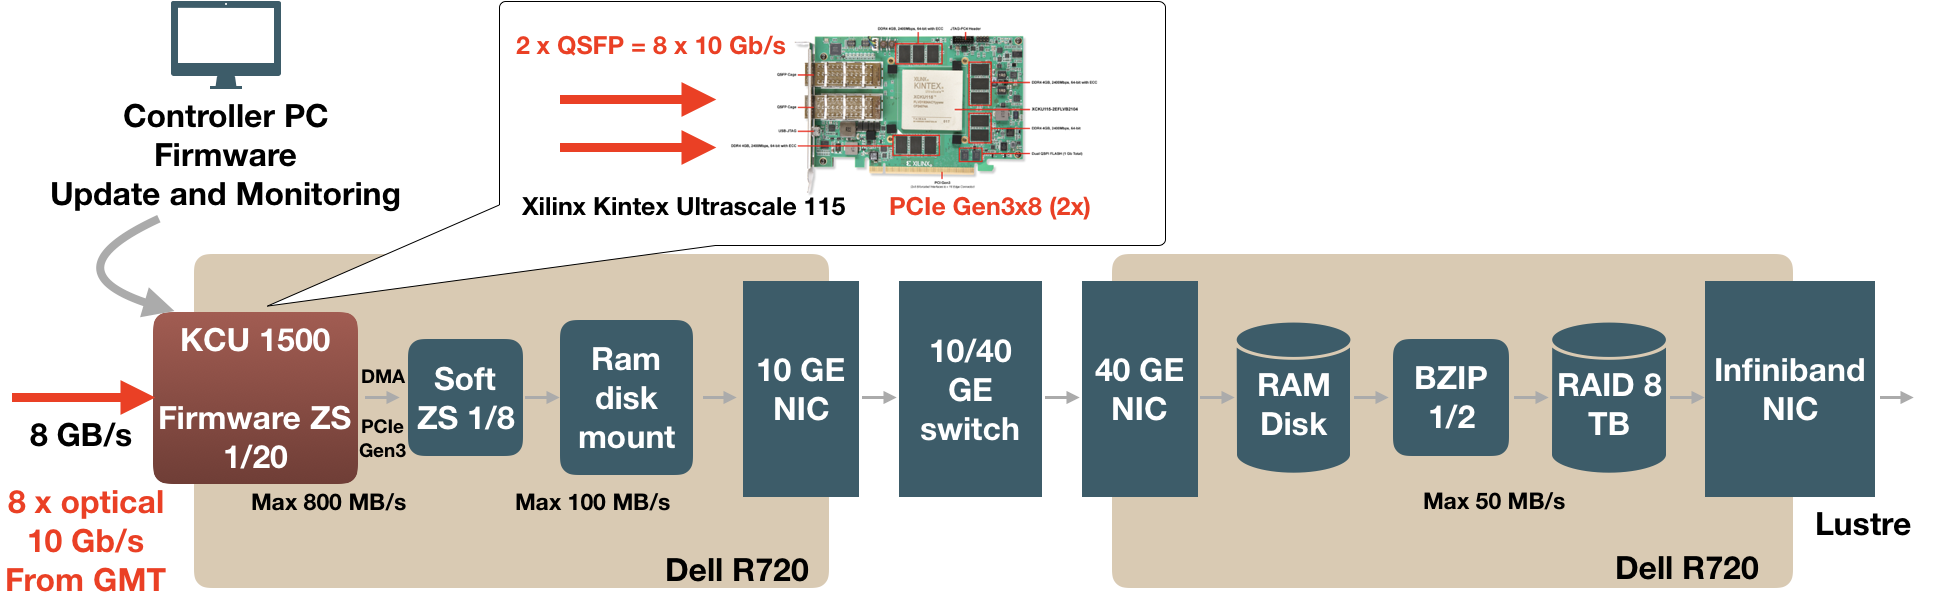
\includegraphics[height=0.2417\linewidth]{./images/scouting_prot_kcu.png}
    \caption{The LHC Run 2 scouting demonstrator system architecture, consisting of two data processing servers; one of which hosts an FPGA-based processing board, the Xilinx KCU1500~\cite{kcu}.}
    \label{fig:scouting_arch}
\end{figure}

\section{Machine/Deep Learning in High Energy Physics}
\label{Machine/Deep Learning in High Energy Physics}

Machine learning (ML) describes a set of algorithms that can perform a specific task without being explicitly programmed to do so. Parameters of machine learning models are learned during the \textit{training}, allowing data to shape and influence the algorithm implementation. Deep learning (DL) is a subset of machine learning algorithms that contain multilayered learning systems, such as neural networks (NN)~\cite{DL}. In principle, any function may be approximated by a NN. Training is performed with the objective of minimizing the model loss (the difference between targets and model predictions).

ML algorithms have been used in High Energy Physics (HEP) for various tasks. For example, widely used classification models can be used for particle identification. ML models can also be used to perform direct measurements of physical quantities from a set of input signals. Unsupervised ML algorithms could be used for clustering problems in HEP. The first applications of neural networks in HEP date back to the 1980s. Starting with the MiniBooNE~\cite{miniboone} experiment, boosted decision trees increased in popularity, and played an important role in the discovery of the Higgs boson by the ATLAS and CMS experiments~\cite{aradovic}. Huge amounts of data, collected during experiments, can be used for training the machine learning models. With the improvement in computing power and the expansion of deep learning accelerators, there is a possibility to apply DL techniques in various stages of data acquisition. Extensive research is performed by multiple groups at CERN, academia~\cite{hls4ml}, industry~\cite{ibm_low_inf}, and the open source community~\cite{qkeras} in order to utilise resource-bound FPGA-based hardware to execute computationally extensive models.


\section{Deep Learning in 40 MHz Scouting}
\label{Deep Learning in 40 MHz Scouting}

\subsection{Problem}
Offline reconstruction, executed at the order of 1 Hz per core, performs complex computations of the muon parameters received from the detector to determine the actual position of muon tracks. The offline reconstruction provides the best possible estimate of the physics event content, within current technological and resource boundaries. With the reconstructed data, a proper physics analysis can be performed. One of the limitations of the offline reconstruction is the duration of execution. It is not feasible to execute such complex algorithms at the 40 MHz BX rate. Unlike the reconstructed objects at the L1 trigger, offline reconstruction contains the complete event information.


As the L1 Trigger objects are optimised for efficiency and rate at the given L1 trigger thresholds, not for a general physics analysis, it is advantageous to apply some corrections and re-calibrations to these objects within the scouting system. One proposal is to utilise DL algorithms to approximate the offline reconstruction of the particles. 

One can train a DL model to predict the offline reconstructed parameters of a given physics object, from matching L1 objects found in historical data. In this way, it is possible to improve the resolution of the L1 objects, in a low-latency environment. While the neural network is not able to provide the full precision of the offline reconstruction, (partially as a result of missing silicon tracker information which is not currently available at 40 MHz), the effects of digitisation and bias in the L1 trigger algorithms can be reduced, particularly in regions of phase space not near the L1 trigger thresholds. 



\subsection{Datasets}

ZeroBias datasets from 2017 and 2018 are used to train the neural networks. These events are not correlated to any particular physics signatures. The L1 muon tracks generated by the L1 Barrel Muon Track Finder (BMTF) are matched to the offline reconstructed muons with a selection of $\Delta R < 0.1 $, as calculated at the second station of the barrel muon detector. Additionally, only L1 muon candidates with $2.5 < p_\mathrm{T} < 45$ GeV are used for training.

\subsection{Model Inputs and Targets}

An L1 trigger muon object is a 64 bit representation of a muon track~\cite{DN2014}. A certain number of bits are assigned to different muon parameters, including $\phi$ and $\eta$, both at the second muon station, and after extrapolation back to the vertex. Additionally, the \textit{p}\textsubscript{T} from the trackfinder, and the muon charge. These parameters are potential inputs to the DL model. Due to the bending of particles in the magnetic field, the values of the track parameters in the muon system, and near the collision point, can be different. In most cases, the extrapolated values are used as an input to the neural network, as the kinematics at the interaction vertex are the most relevant for physics analysis.

\subsection{Baseline Model}
The baseline model used is a multilayered perceptron with the following characteristics:

\begin{itemize}

    \item Four input parameters, and three output parameters. The overall size of the network is limited by the low number of inputs and outputs, and the fact that the models will be synthesised on the resource restricted hardware. The baseline model has three hidden layers, with 32 nodes per layer.
    
    \item The activation function in the hidden layers is \textit{relu}, and linear in the output layers.

    \item Batch normalization (BN)~\cite{bn} is used before each activation in the hidden layers.

    \item The model inputs are integer values from the L1 trigger muon objects: $\phi$, $\eta$, \textit{p}\textsubscript{T}, and charge sign. Before training and inference, the inputs are normalized to the range [0-1].

    \item The prediction targets are three float values from the offline reconstructed muons. The model targets are three float values representing the difference between the L1 and reconstructed parameters; $\phi$, $\eta$ and \textit{p}\textsubscript{T}). Before training, the target outputs are also normalised to the range [0-1].
    
    \item The optimizer is \textit{Adam}~\cite{Adam}, with the default parameters. The loss function is mean squared error.

\end{itemize}

\subsection{Evaluation Metrics}

%TJ comment - clarify GMT vs BMTF - first time using GMT here?

In order to determine if the NN approach improves upon the resolution provided by the Global Muon Trigger (GMT), the distribution of differences between the GMT outputs and the offline reconstructed values is compared to the distribution of differences between the neural network outputs and the offline reconstructed values. Three metrics are used to compare model performance. 

\begin{itemize}
\item The root mean square (RMS). With this metric, the width of the distributions is compared. To demonstrate the resolution improvement, this metric would show narrower neural network difference distribution compared to the GMT difference distribution.

\item The percentage of data in the distribution core. The distribution core is defined as $\pm\,8$\,mrad, $\pm\,0.0015$, and $\pm\,10$\,MeV around zero for $\phi$, $\eta$, and $p_\mathrm{T}$ respectively. A higher percentage of data in the core represents an improvement in the difference distribution.

\item The percentage of data in the distribution tails. The distribution tails are ranges of significant difference between the observed output (GMT or the neural network) and the offline reconstructed values. For $\phi$, the data are considered to be in the tail if the absolute difference is more than 0.1 radians. For $\eta$, the data are considered to be in the tail if the absolute difference is more than 0.05. For \textit{p}\textsubscript{T}, the data are considered to be in the tail if the absolute difference is greater than 15\% of the reconstructed $p_\mathrm{T}$. A lower percentage of data in the tails of the neural network difference distribution would demonstrate an improvement.

\end{itemize}

\subsection{Hyper-parameter Optimization}

Hyper-parameters are parameters of the model that are not learned during training. It is important to perform an optimisation of these parameters, in order to find the configuration of the model that produces the best results. In this work, an incremental approach is conducted. The initial, baseline model is created, and various options to improve its results are evaluated. Some of the hyper-parameters to optimise are: the number of layers, the number of nodes in each layer, the loss function, the loss weights, the learning rate, the optimizer, the regularization, and the activation functions. For evaluation, a five-fold cross validation was used. The models were implemented using the Keras~\cite{keras} framework.

Multiple loss functions were tested: mean squared error, mean squared logarithmic error, and logcosh. A variety of Keras optimizers were tested: Adam, SGD, Adadelta and Adagrad~\cite{optimizers_overview}.

Regularization is a technique which prevents models from over-fitting by introducing a small penalty in the training. This also improves training stability. L1 and L2 regularization functions~\cite{andrewng_reg} were tested, with parameters (10\textsuperscript{-5}, 10\textsuperscript{-7} and 10\textsuperscript{-9}).

The relu activation function was tested in the output layer, but it was unsuccessful in comparison to a linear function. In the hidden layers softmax and relu activation functions were tested, with similar results.

\begin{table}[!htb]
\setlength{\belowcaptionskip}{-10pt}
  \begin{center}
    \begin{tabular}{|>{\centering\arraybackslash}p{0.4cm}|c|c|c|c|c|c|c|c|c|}
      \hline
      Id & Loss function & Optimizer & Regularization & Activation HL & Activation OL \\
      \hline
      A & logcosh & Adam & None & Relu & Linear \\
      \hline
      B & logcosh & Adadelta & None & Relu & Linear \\
      \hline
      C & logcosh & Adadelta & L2 $\lambda$=10\textsuperscript{-7} & Relu & Linear \\
      \hline
      D & logcosh & Adadelta & L2 $\lambda$=10\textsuperscript{-9} & Relu & Linear \\
      \hline
      E & logcosh & Adam & L2 $\lambda$=10\textsuperscript{-7} & Relu & Linear \\
      \hline
      F & logcosh & Adam & None & Softmax & Linear \\
      \hline
    \end{tabular}
    \caption{A description of a some of the most promising models that were tested. The activation functions in the hidden layers (HL) and output layers (OL) are given, alongside the loss functions and optimiser of choice for models labelled A-F.}
    \label{tab:model_settings}
  \end{center}
\end{table}

\begin{table}[!htb]
\setlength{\belowcaptionskip}{-10pt}
  \begin{center}
    \begin{tabular}{|>{\centering\arraybackslash}p{0.75cm}|>{\centering\arraybackslash}p{1.3cm}|>{\centering\arraybackslash}p{1.3cm}|>{\centering\arraybackslash}p{1.3cm}|>{\centering\arraybackslash}p{1.3cm}|>{\centering\arraybackslash}p{1.3cm}|>{\centering\arraybackslash}p{1.3cm}|>{\centering\arraybackslash}p{1.3cm}|>{\centering\arraybackslash}p{1.3cm}|>{\centering\arraybackslash}p{1.3cm}|}
      \hline
      & \multicolumn{3}{c|}{RMS} & \multicolumn{3}{c|}{Data in the core [\%]} & \multicolumn{3}{c|}{Data in the tail [\%]}\\
      \hline
      Id & $\Delta\phi$ & $\Delta\eta$ & $\Delta$\textit{p}\textsubscript{T}/\textit{p}\textsubscript{T}\textsubscript{r} & $\Delta\phi$ & $\Delta\eta$ & $\Delta$\textit{p}\textsubscript{T}/\textit{p}\textsubscript{T}\textsubscript{r} & $\Delta\phi$ & $\Delta\eta$ & $\Delta$\textit{p}\textsubscript{T}/\textit{p}\textsubscript{T}\textsubscript{r}\\
      \hline
	  GMT & 0.166 & 0.034 & 0.274 & 14.82 & 4.86 & 10.54 & 41.25 & 15.14 & 44.84 \\ 
	  \hline
	  A & 0.120 & \bf{0.031} & 0.169 & \bf{20.17} & 5.28 & 14.20 & 27.07 & 11.55 & 28.29 \\ 
	  \hline
	  B & 0.119 & \bf{0.031} & 0.167 & 19.75 & 5.29 & 14.76 & 26.79 & \bf{11.45} & 26.68 \\ 
	  \hline
	  C & 0.119 & \bf{0.031} & \bf{0.165} & 19.37 & 5.29 & \bf{14.85} & 26.90 & 11.58 & 26.62 \\ 
	  \hline
	  D & \bf{0.117} & \bf{0.031} & 0.167 & 19.56 & 5.27 & 14.70 & \bf{26.73} & 11.54 & 26.84 \\ 
	  \hline
	  E & 0.118 & \bf{0.031} & 0.167 & 20.16 & \bf{5.34} & 14.61 & 26.85 & 11.50 & 27.04 \\ 
	  \hline
	  F & 0.119 & \bf{0.031} & 0.167 & 19.61 & 5.24 & 14.76 & 26.89 & 11.54 & \bf{26.48} \\ 
	  \hline
    \end{tabular}
    \caption{The results of the model configurations described in Tab.~\ref{tab:model_settings}. The $\Delta$ values refer to the difference between the predicted $\phi$, $\eta$, or $p_\mathrm{T}$ and the offline reconstructed values. The $p_\mathrm{T}$ distribution is divided by the offline reconstructed $p_\mathrm{T}$ ($p_\mathrm{Tr}$). The best result for a each metric is given in bold. }
    \label{tab:hp_results}
  \end{center}
\end{table}

\subsection{Deep Learning Results}

The results of the models defined in Tab.~\ref{tab:model_settings} are shown in Tab.~\ref{tab:hp_results}. It is observed that each of the models provides an improvement compared to the GMT outputs. Models' results show reduced RMS for the three output variables ($\phi$, $\eta$, \textit{p}\textsubscript{T}). The percentage of data in the core, and the amount of data in the tails, is also reduced, however, the difference between the results of each NN model shown in Tab.~\ref{tab:model_settings} is small. There is no single model which shows the best performance across all metrics and output variables; for each metric a different set of hyper-parameters produces the best performance. For example, considering the percentage of data in the distribution core, the best performance for $\phi$ is shown by the model A, for $\eta$ by the model E and for \textit{p}\textsubscript{T} by model C. Similarly, models D, B and F produce the least amount of data in the tails. Model B is used for the further analysis described in this paper.

Figure~\ref{fig:residuals} shows the distribution of differences between the model predictions and the offline reconstructed values in shown in red; and the distribution of differences between GMT values and the offline reconstructed values in blue. As expected, the neural network outputs produce a narrower distribution around zero.
 
%%%%%%%%%%%%%%%%%%%%%%%%%%%%%%%%%%%%%%%%%%%%%%%%%%%%%%%%%%%%%%%%%%%%%%%%%
%%   use this format to include an .eps or .pdf figure(s) into your paper
%%%%%%%%%%%%%%%%%%%%%%%%%%%%%%%%%%%%%%%%%%%%%%%%%%%%%%%%%%%%%%%%%%%%%%%%%

% set the height or width as you prefer
\begin{figure}[!htb]
  \centering
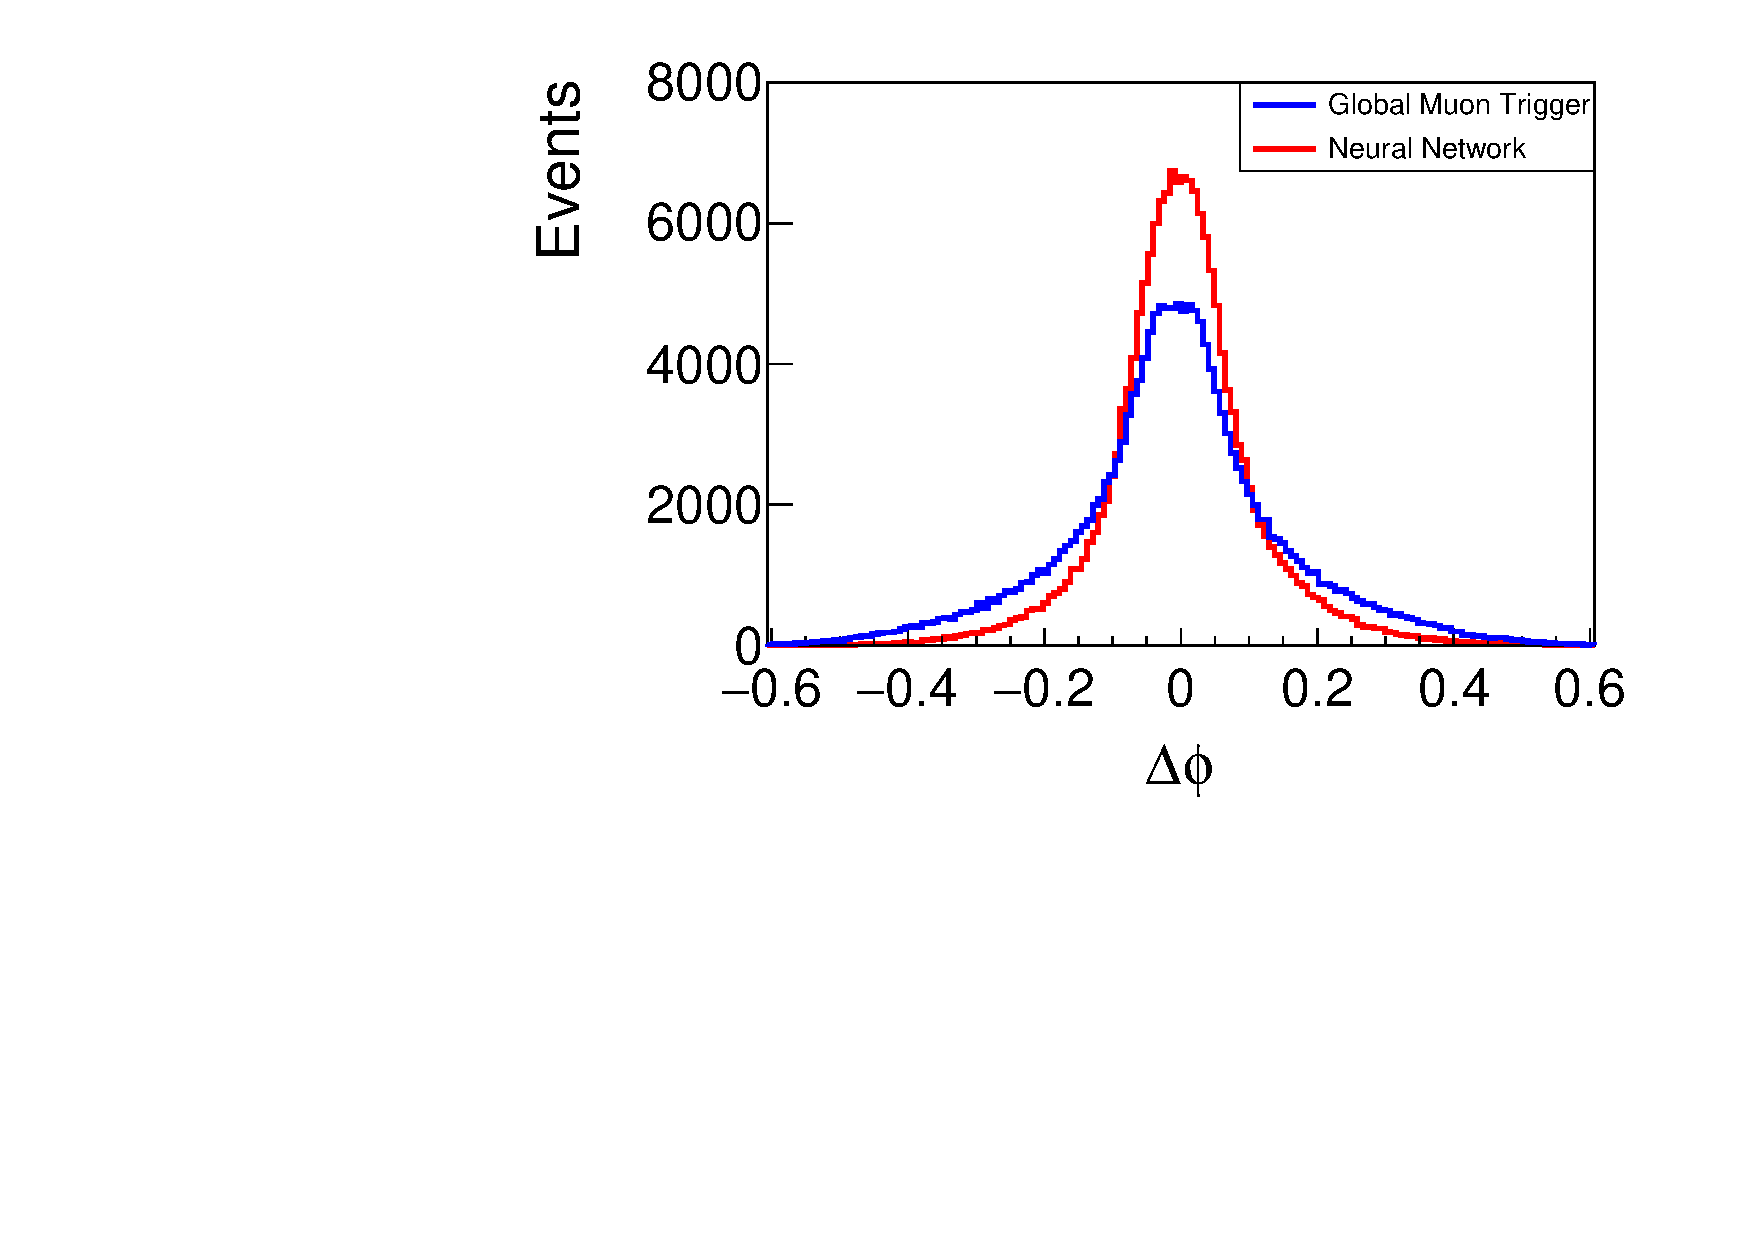
\includegraphics[width=0.31\linewidth]{./images/delta_phi_no_gauss_GMT_pt_cut.pdf}
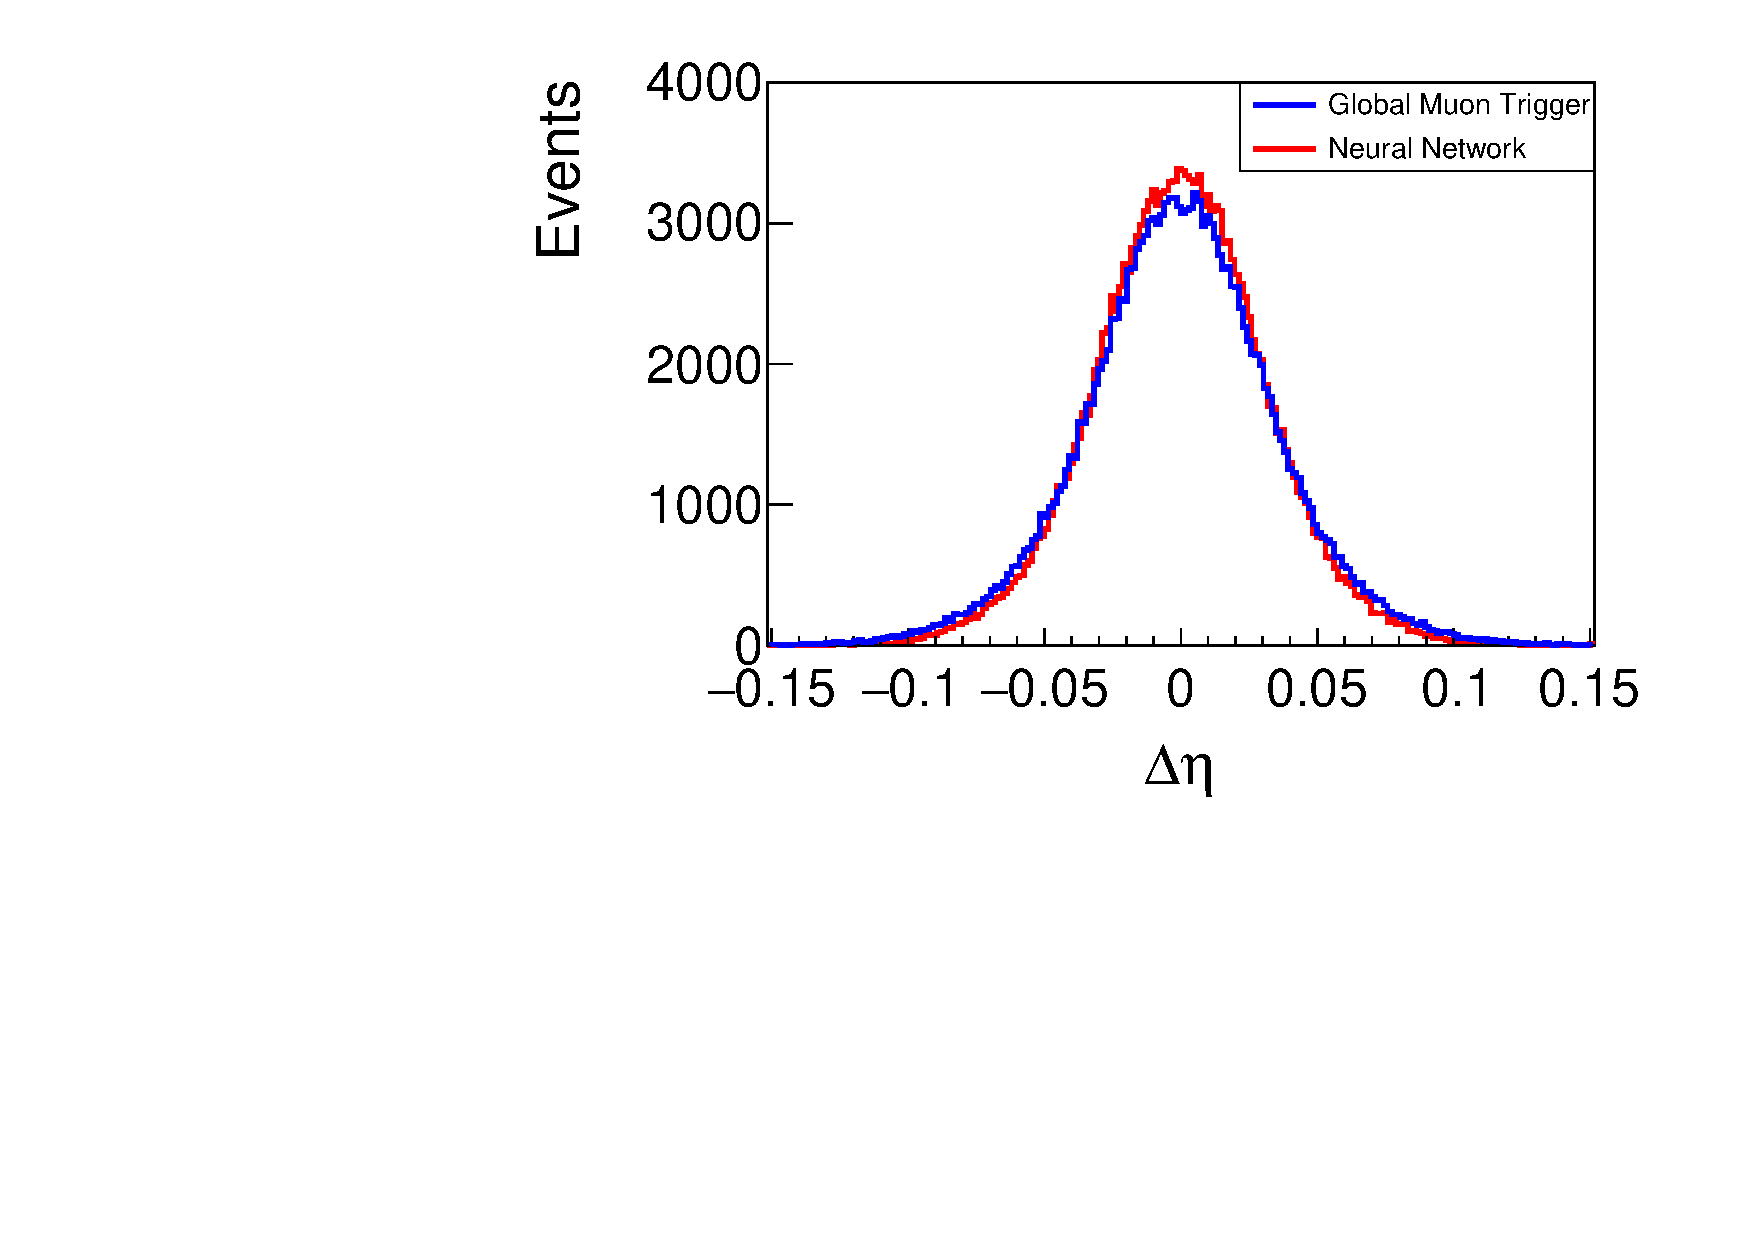
\includegraphics[width=0.31\linewidth]{./images/delta_eta_no_gauss_GMT_pt_cut.pdf}
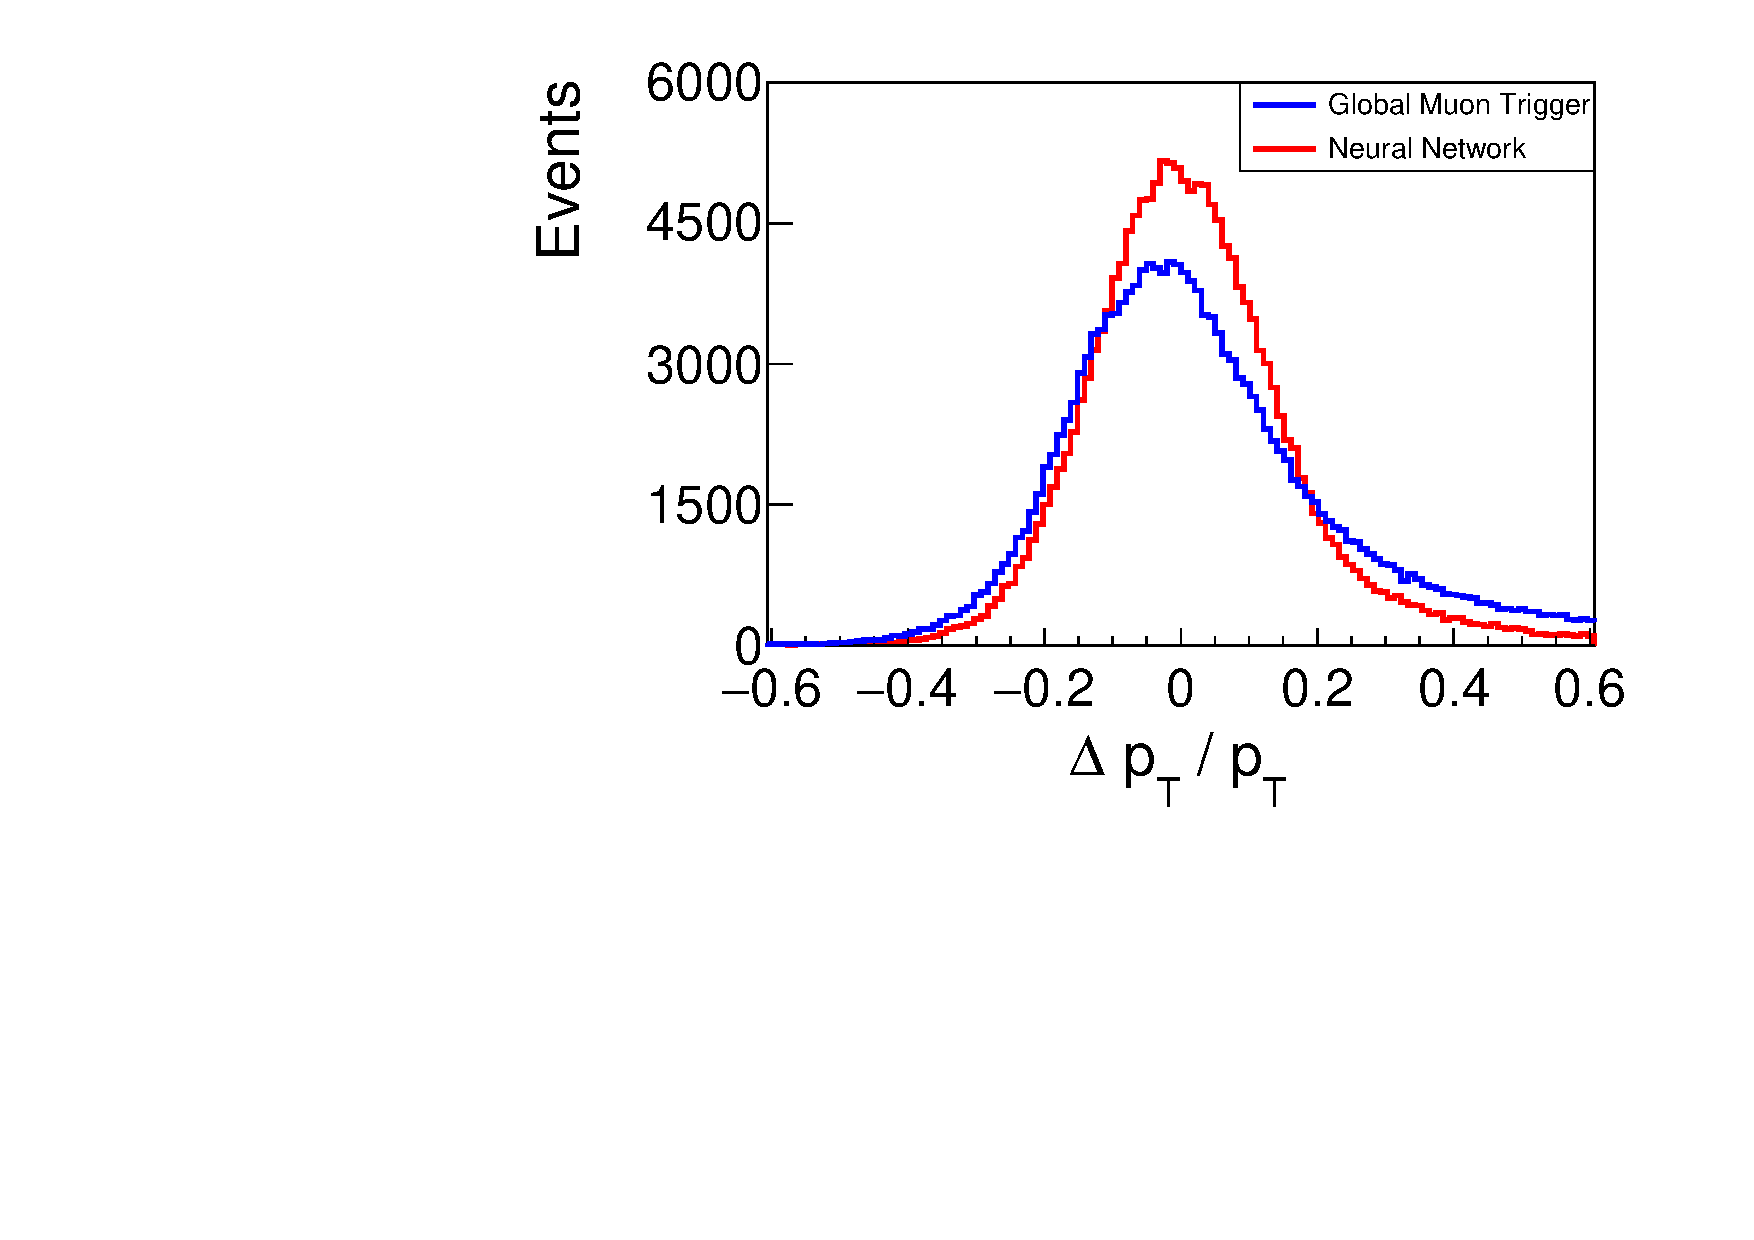
\includegraphics[width=0.31\linewidth]{./images/delta_pt_over_pt_no_gauss_GMT_pt_cut.pdf}
  \caption{The difference between GMT and offline reconstructed values of $\phi$, $\eta$, and $p_\mathrm{T}$ (blue), compared to the difference between the NN predictions and reconstructed values (red). GMT muons with a $p_\mathrm{T}$ estimate below 3 GeV are excluded, as a high fraction of unwated duplicate muon candidates were found between 2.5 and 3 GeV.}
  \label{fig:residuals}
\end{figure}

%The Figure~\ref{fig:pt_range} shows the affect of the neural network correction with respect to the \textit{p}\textsubscript{T} range. The x-axis shows an offline reconstructed \textit{p}\textsubscript{T} range. The y-axis shows the mean absolute difference between the output values (model or GMT) and the offline reconstructed values, in a range represented by a histogram bin. The plot shows that the neural network improves the resolution on a significant part of the \textit{p}\textsubscript{T} range. 

%commented out by tjames to reduce length to 6 page recommendation
%\begin{figure}[!htb]
%    \centering
%    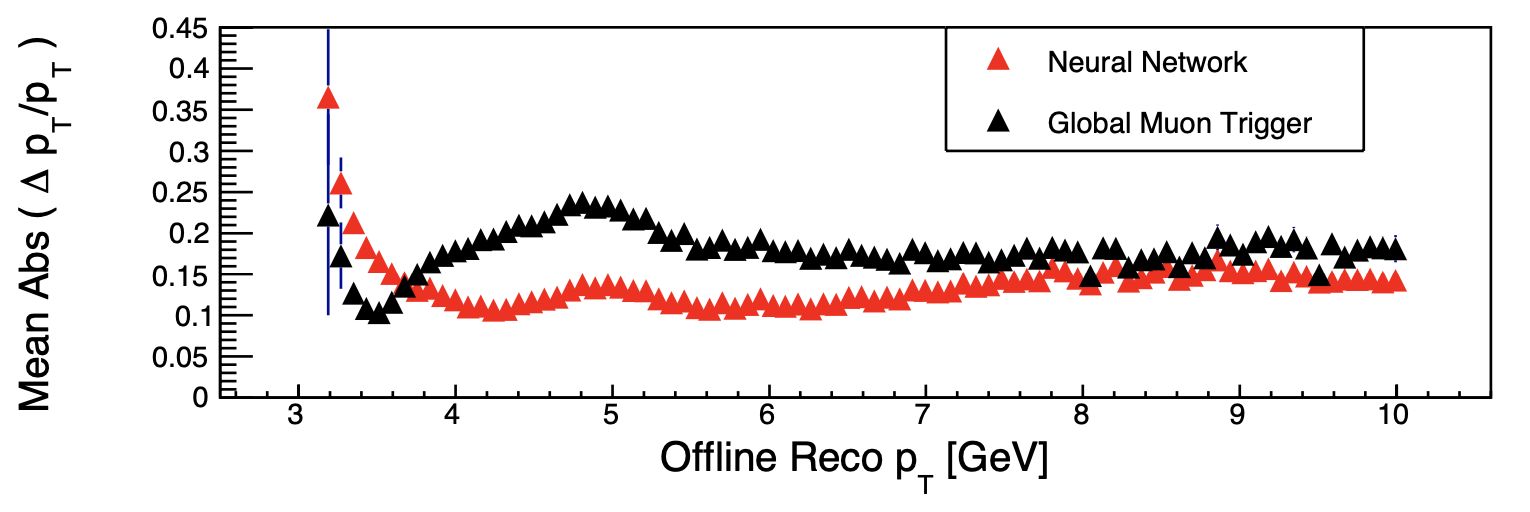
\includegraphics[width=1\linewidth]{./images/gmt_range_2.png}
%    \caption{ZeroBias datasset, comparison between neural network and GMT, on the \textit{p}\textsubscript{T} range.}
%    \label{fig:pt_range}
%\end{figure}





\begin{figure}[!htb]
    \centering
    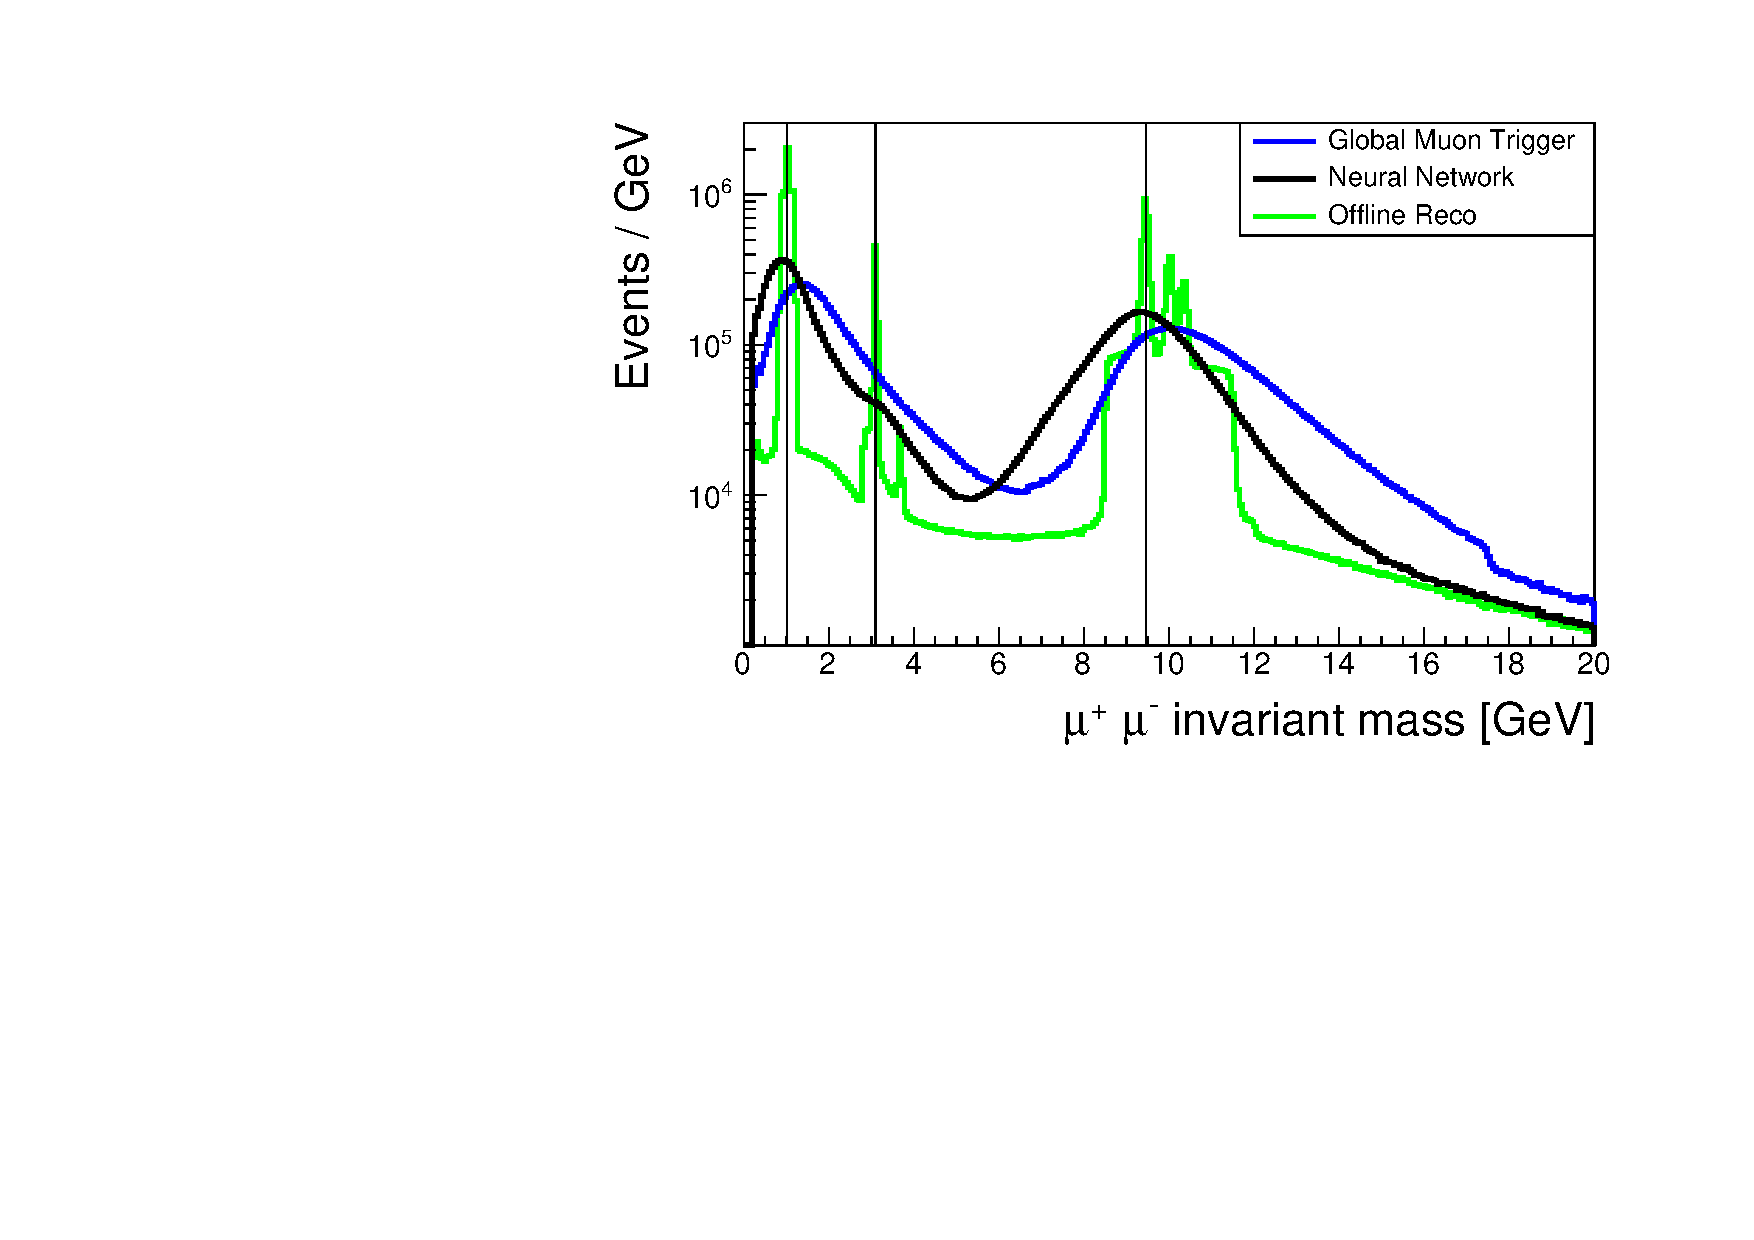
\includegraphics[width=0.72\linewidth]{./images/inv_mass_total_lines_2.pdf}
    \caption{Invariant mass distribution of muon pairs, produced by the CMS MuOnia 2018 dataset.}
    \label{fig:inv_mass}
\end{figure}

%Commented out by TJ to save space, can discuss
%\begin{figure}[!htb]
%  \centering
%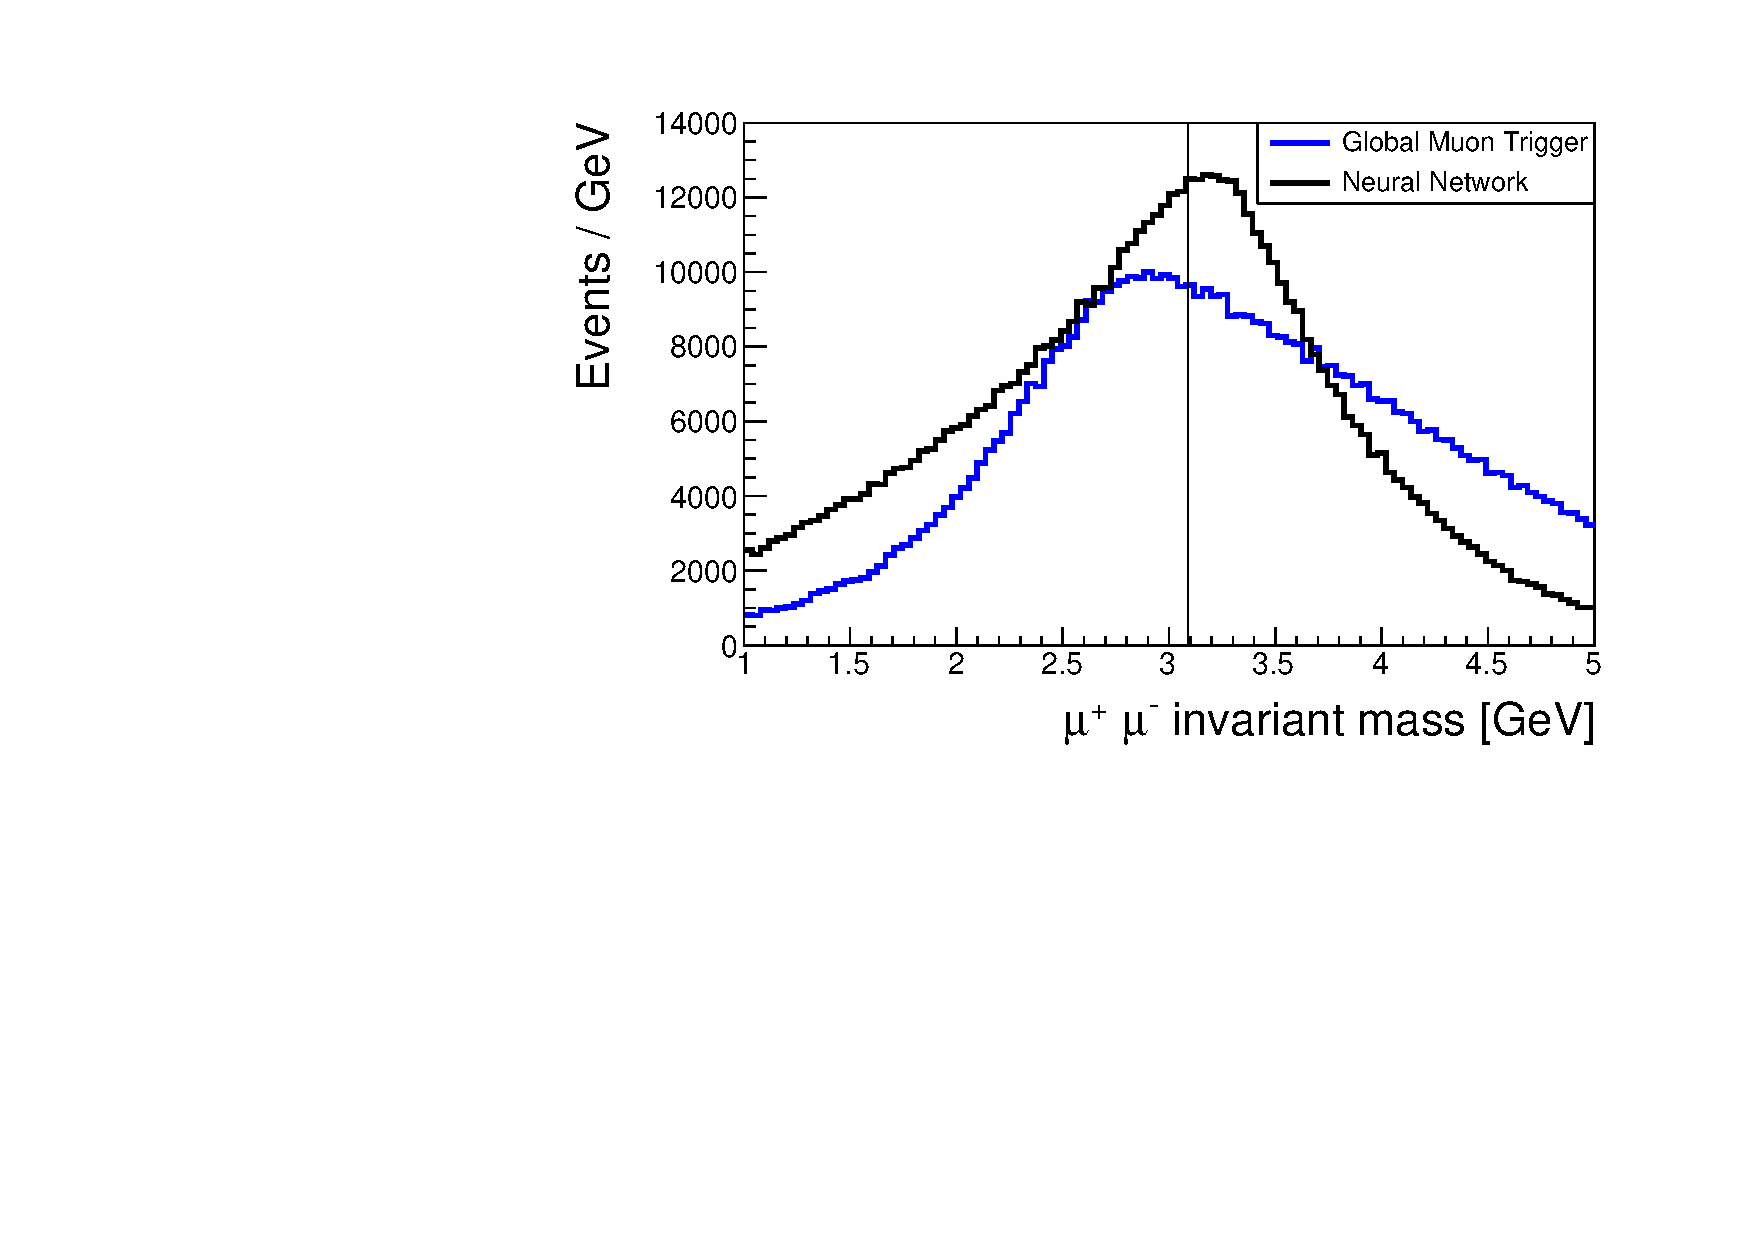
\includegraphics[width=0.4\linewidth]{./images/inv_mass_total_3_lines.pdf}
%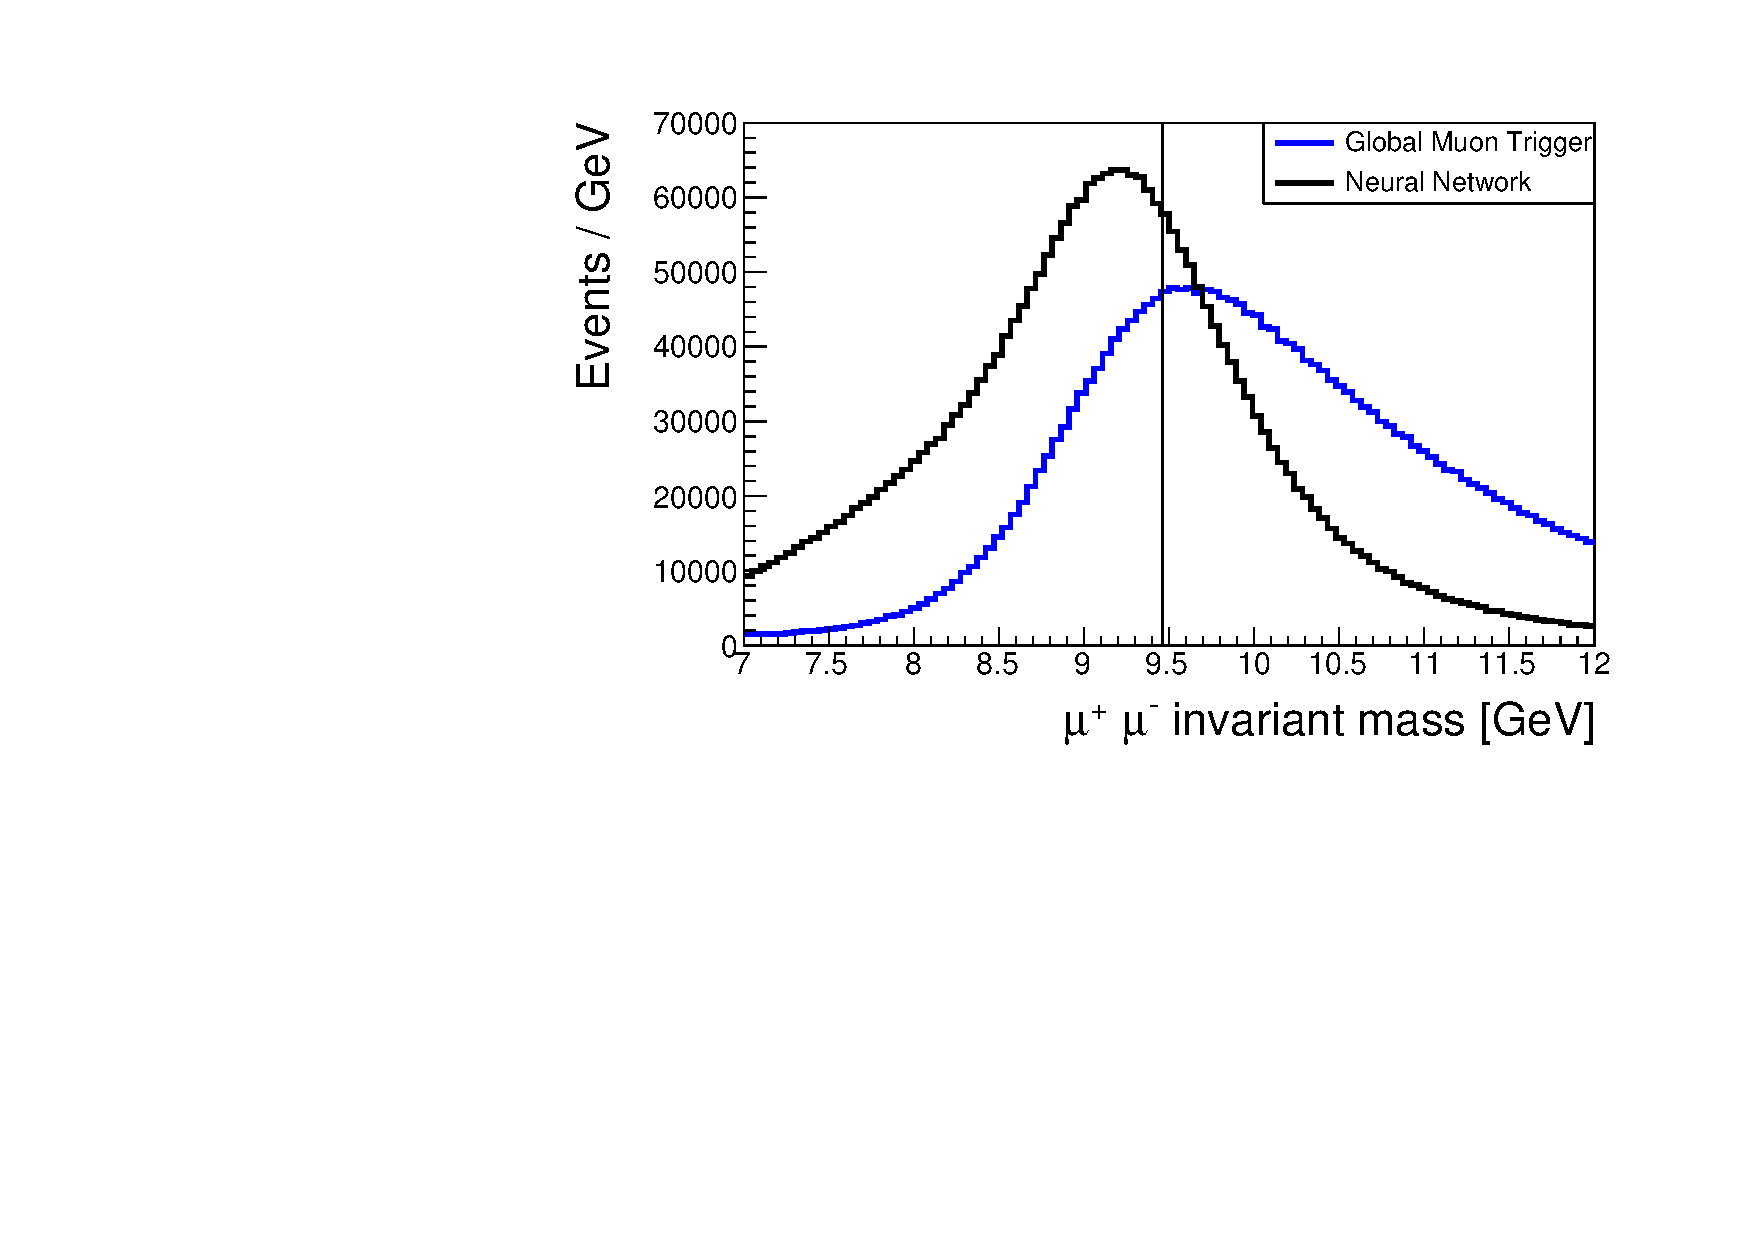
\includegraphics[width=0.4\linewidth]{./images/inv_mass_total_9_lines.pdf}
%  \caption{Invariant mass distribution of muon pairs around J/$\psi$ resonance (left), and the $\Upsilon$ resonance (right). Selection cuts on the invariant mass calculated with the offline tracks of $2 < m_\mathrm{inv} < 5$ GeV (left), and $7 < m_\mathrm{inv} < 12$ GeV (right) were also applied. Produced with the MuOnia dataset from 2018.}
%  \label{fig:inv_mass_ranges}
%\end{figure}

To evaluate the performance of this DL approach in the context of muon pairs, the MuOnia dataset from 2018 was used. This dataset consists of HLT selected events containing opposite-charge muon pairs and can therefore be used to produce an invariant mass distribution that includes a series of narrow resonances. As shown in Fig.~\ref{fig:inv_mass}, the invariant mass distribution in the range $0\,<\,m_\mathrm{inv}\,<\,20$\,GeV is calculated using three different sets of values: GMT outputs, the NN outputs, and the offline reconstructed values. Vertical lines in this plot correspond to known particle mass resonances; the $\phi$ meson, J/$\psi$ meson, and $\Upsilon$ meson with respective masses of 1.02, 3.09 and 9.46 GeV. As expected, the most precise results are achieved using the offline reconstructed values, and the least precise with the GMT output. The NN outputs, show a resolution in-between the GMT and reconstructed values. Although the neural network result is unable to distinguish resonances within a particle family, the peaks are narrower and closer to the true values that for the GMT; additionally a bump can be observed around the J/$\psi$ meson resonance, which can not be seen in the original GMT data.

%Commented out by TJ to save space, can discuss
%Figure~\ref{fig:inv_mass_ranges} represents the distribution of invariant mass produced by the GMT and the neural network. These plots were produced using muons where the offline reconstructed invariant mass is within the ranges of [2 - 5] and [8 - 12] GeV. The plots show the that the neural network improves the height of the distribution. The central value is also improved.

\subsection{Deep Learning on Hardware}

The scouting system requires that the DL models are implemented in field-programmable gate array (FPGA) firmware. The high bandwidth required excludes the use of CPUs or GPUs. Implementing deep learning algorithms using hardware description languages such as VHDL or Verilog is a challenging and a time-consuming task. Even though the custom implementation may achieve the best performance in terms of FPGA resource utilisation, it is not an efficient solution when the field of deep learning is rapidly evolving. Since deep learning algorithms are implemented using high-level programming languages (mainly Python), we plan to use a compiler which would translate the Python developed models into the instructions for the FPGA-based hardware.

The hardware used for the implementation of the developed deep learning models are the Micron SB-852 and Micron AC-510 FPGA-based processing boards~\cite{micron_company}~\cite{micron_sb852}~\cite{micron_ac510}. The SB-852 contains the Xilinx Virtex Ultrascale+ UV9P FPGA~\cite{vu9p}, 64GB DDR4 memory, two QSFP optical link interfaces and a PCIe x16 Gen3 connector to the host. The board is installed in one of the CMS servers for testing purposes.

Compiling the deep learning models developed in Python is done using the Micron Deep Learning Accelerator (MDLA)~\cite{micron_sdk}. The MDLA allows access to the board from the host using Python programming language, providing an easy way to evaluate a variety of deep learning models on the FPGA-based board. The implementation is hidden from the user, eliminating any need to write low level code or firmware for the deep learning models. The development process starts with model training in one of the Python frameworks such as Keras~\cite{keras}, TensorFlow~\cite{tf} and PyTorch~\cite{pytorch}. Then, the models are converted to the Open Neural Network Exchange (ONNX)~\cite{onnx} format. After the conversion, the MDLA API is used to communicate with the board, in order to set-up the model execution in the FPGA. Information about the models is sent to the board, where multiple computational clusters are initiated to perform assigned deep learning operations~\cite{mircon_paper_1}~\cite{mircon_paper_2}. The configuration includes the size of the inference batch, the number of computational clusters, the path to the model files and the other options. After that, an inference can be performed. During the evaluation period, various information about inference performance has been measured, including latency and throughput.

The objective is to have a throughput of 10\textsuperscript{6} inferences per second. As shown in Table \ref{tab:DLA_perf}, the performance achieved using the MDLA satisfies the requirements. Using two computational clusters within a single AC-510 board, the requirements are exceeded by almost a factor of three. With the expected future upgrades of the MDLA hardware and software, an increase in performance is expected. The results obtained should allow for the inclusion of the Micron hardware in the scouting system, replacing the KCU1500 board.

\begin{table}[!htb]
\setlength{\belowcaptionskip}{-20pt}
  \begin{center}
    \begin{tabular}{|c|c|c|c|}
      \hline
      Hardware & Clusters & Latency [ns] & Inferences per second \\
      \hline
      AC-510 & 1 & 726 & \textgreater~1 300 400 \\
      \hline
      AC-510 & 2 & 364 & \textgreater~2 700 000 \\
      \hline
      SB-852 & 1 & 748 & \textgreater~1 300 000 \\
      \hline
    \end{tabular}
    \caption{Scouting neural network (Model B) performance on the MDLA, with the AC-510 and SB-852 FPGA-based boards.}
    \label{tab:DLA_perf}
  \end{center}
\end{table}

\section{Summary and Outlook}

Correcting L1 muon objects using deep learning models shows potential for further use within the CMS L1 scouting system. It has been established that the use of deep learning models improves the resolution of the invariant mass of pairs of muons. The deep learning models are implemented in FPGA-based hardware, and the measured throughput and latency fit into the CMS scouting requirements. The MDLA will now be integrated into the scouting system for LHC Run-3; and new models will developed to take advantage of additional inputs to the L1 scouting system.

\Acknowledgements
We thank Micron Technology Inc. for the financial contribution and the technical support throughout the project. We thank CMS EP-CMG group for the collaboration and the valuable insights during the project.

%%%%%%%%%%%%%%%%%%%%%%%%%%%%%%%%%%%%%%%%%%%%%%%%%%%%%%%%%%%%%%%%%%%%%%%%%%%
%%%%%%%%%%%%%%%%%%%%%%%%%%%%%%%%%%%%%%%%%%%%%%%%%%%%%%%%%%%%%%%%%%%%%%%%%%%

\begin{thebibliography}{99}

%%
%%  bibliographic items can be constructed using the LaTeX format in SPIRES:
%%    see    http://www.slac.stanford.edu/spires/hep/latex.html
%%  SPIRES will also supply the CITATION line information; please include it.
%%

%\bibitem{lhc}
%  L. Evans, P. Bryant et al.,
%  “LHC machine",
%  JINST {\bf 3}, S08001, (2008),
%  doi:10.1088/1748-0221/3/08/s08001.

\bibitem{tdr}
  The CMS Collaboration, 
  “The Phase-2 Upgrade of the CMS Level-1 Trigger”,
  CERN/LHCC (to be published).
    
\bibitem{trigger}
  The CMS Collaboration,
  “The CMS trigger system",
  JINST {\bf 12}, P01020, (2017),
  doi:10.1088/1748-0221/12/01/p01020.

\bibitem{duarte2018fast}
  J. Duarte
  “Fast Reconstruction and Data Scouting",
  Proceedings of Connecting the Dots, (2018),
  arXiv:1808.00902.

\bibitem{dustin}
  D. Anderson (CMS),
  “Data Scouting in CMS",
  Proceedings of 38th International Conference on High Energy Physics (ICHEP), Chicago, IL, USA, (2016).

\bibitem{hannes} 
  H. Sakulin et al.,
  “40 MHz Level-1 Trigger Scouting for the Compact Muon Solenoid Experiment",
  Proceedings of 24th International Conference on Computing in High-Energy and Nuclear Physics, Adelaide, Australia, (2019).
  
\bibitem{BRIL}
  The CMS Collaboration,
  “The Phase-2 Upgrade of the CMS Beam Radiation, Instrumentation, and Luminosity Detectors: Conceptual Design”,
  (2020).

\bibitem{kcu}
  Xilinx Inc.,
  \url{www.xilinx.com/products/boards-and-kits/dk-u1-kcu1500-g.html},
  [Accessed 2020-02-26].
  
\bibitem{ku115}
  Xilinx Inc.,
  \url{www.xilinx.com/products/silicon-devices/fpga/kintex-ultrascale.html},
  [Accessed 2020-03-05].

\bibitem{bzip}
  J. Seward,
  “bzip2",
  \url{www.sourceware.org/bzip2},
  [Accessed 2020-02-26].

\bibitem{lustre}
  "Lustre",
  \url{www.lustre.org},
  [Accessed 2020-03-12].
  
\bibitem{DL}
  Y. Bengio, Y. LeCun, G. Hinton,
  “Deep Learning",
  Nature {\bf 521}, 436–444, (2015),
  doi:10.1038/nature14539.
  
\bibitem{miniboone}
  A. A. Aguilar-Arevalo  et al,
  “The MiniBooNE Detector”,
  Nuclear Instruments and Methods in Physics Research Section A: Accelerators, Spectrometers, Detectors and Associated Equipment {\bf 599.1}, 28–46, (2009),
  doi:10.1016/j.nima.2008.10.028.

\bibitem{aradovic}
  A. Radovic et al.,
  “Machine learning at the energy and intensity frontiers of particle physics",
  Nature {\bf 560}, 41–48, (2018),
  doi:10.1038/s41586-018-0361-2.
  
\bibitem{hls4ml}
  J. Duarte, S. Han, P. Harris, S. Jindariani, E. Kreinar, B. Kreis, J. Ngadiuba, M. Pierini, R. Rivera, N. Tran, Z. Wu,
  “Fast inference of deep neural networks in FPGAs for particle physics",
  (2018),
  doi:10.1088/1748-0221/13/07/p07027.
  
\bibitem{ibm_low_inf}
  S. Gupta, A. Agrawal, K. Gopalakrishnan, P. Narayanan,
  “Deep Learning with Limited Numerical Precision",
  (2016),
  arXiv:1502.02551.
  
\bibitem{qkeras}
  “QKeras",
  \url{www.github.com/google/qkeras/blob/master/README.md},
  [Accessed 2020-03-05].
  
\bibitem{DN2014}
  The CMS Collaboration,
  “Scales for inputs to $\mu$GT ($\phi$, $\eta$, \textit{p}\textsubscript{t}/\textit{E}\textsubscript{t}), and others",
  \url{http://globaltrigger.hephy.at/files/upgrade/ugt/scales_inputs_2_ugt_2017Aug14.pdf},
  [Accessed 2020-03-09].
  
\bibitem{bn}
  S. Ioffe, C. Szegedy,
  "Batch Normalization: Accelerating Deep Network Training by Reducing Internal Covariate Shift",
  (2015),
  arXiv:1502.03167.
  
\bibitem{Adam}
  D. P. Kingma, J. Ba,
  “Adam: A Method for Stochastic Optimization",
  (2014),
  arXiv:1412.6980.
  
\bibitem{keras}
  “Keras",
  \url{www.keras.io},
  [Accessed 2020-03-09].

\bibitem{optimizers_overview}  
  S. Ruder,
  “An overview of gradient descent optimization algorithms",
  (2016),
  arXiv:1609.04747.
  
\bibitem{andrewng_reg}
  A. Y. Ng,
  “Feature selection, L1 vs. L2 regularization, and rotational invariance",
  International Conference on Machine Learning (ICML), (2004),
  doi:10.1145/1015330.1015435.
  
\bibitem{micron_company}
  Micron Technology, Inc.,
  \url{www.micron.com},
  [Accessed 2020-03-09].
  
\bibitem{micron_sb852}
  Micron Technology, Inc.,
  \url{www.micron.com/products/advanced-solutions/advanced-computing-solutions/hpc-single-board-accelerators/sb-852},
  [Accessed 2020-02-26].
  
\bibitem{micron_ac510}
  Micron Technology, Inc.,
  \url{www.micron.com/products/advanced-solutions/advanced-computing-solutions/ac-series-hpc-modules/ac-510},
  [Accessed 2020-03-09].
  
\bibitem{vu9p}
  Xilinx Inc.,
  \url{www.xilinx.com/products/silicon-devices/fpga/virtex-ultrascale-plus.html},
  [Accessed 2020-03-09].
 
\bibitem{micron_sdk}
  Micron Technology, Inc.,
  “Micron Deep Learning Accelerator Software Development Kit",
  \url{www.github.com/FWDNXT/SDK},
  [Accessed 2020-03-09].
  
\bibitem{tf}
  “Tensorflow",
  \url{www.tensorflow.org},
  [Accessed 2020-03-09].
  
\bibitem{pytorch}
  “Pytorch",
  \url{www.pytorch.org},
  [Accessed 2020-03-09].
  
\bibitem{onnx}
  “Open Neural Network Exchange format (ONNX)",
  \url{www.onnx.ai},
  [Accessed 2020-03-02].
  
\bibitem{mircon_paper_1}
  V. Gokhale, A. Zaidy, A. X. M. Chang, E. Culurciello
  “Snowflake: A Model Agnostic Accelerator for Deep Convolutional Neural Networks",
  (2017),
  arXiv:1708.02579.
  
\bibitem{mircon_paper_2}
  A. X. M. Chang, A. Zaidy, M. Vitez, L. Burzawa, Eugenio Culurciello,
  “Deep neural networks compiler for a trace-based accelerator",
  Journal of Systems Architecture {\bf 102}, 101659, (2020),
  doi:10.1016/j.sysarc.2019.101659.

\bibitem{q8.8}
  ARM Limited,
  “ARM Developer Suite AXD and armsd Debuggers Guide",
  Chapter 4.7.9. AXD \textgreater~AXD Facilities \textgreater~Data formatting \textgreater~Q-format
  (1999-2001),
  ARM DUI 0066D.

\bibitem{kbmtf}
  M. Bachtisa, C. Foudasb, P. Katsoulisb, T. Lama, S. Malliosb, G. Karathanasisc, I. Papavergouc, S. Regnarda, M. Teppera, P. Sphicasc, C. Vellidis,
  “Upgrade of the CMS Barrel Muon Track Finder for HL-LHC featuring a Kalman Filter algorithm and an ATCA Host Processor with Ultrascale+ FPGAs",
  Topical Workshop on Electronics for Particle Physics (TWEPP2018), Antwerp, Belgium, (2018),
  doi:10.22323/1.343.0139.

\end{thebibliography}

%%%%%%%%%%%%%%%%%%%%%%%%%%%%%%%%%%%%%%%%%%%%%%%%%%%%%%%%%%%%%%%%%%%%%%%%%%%
%%%%%%%%%%%%%%%%%%%%%%%%%%%%%%%%%%%%%%%%%%%%%%%%%%%%%%%%%%%%%%%%%%%%%%%%%%%

\end{document}